% This file was created with tikzplotlib v0.10.1.
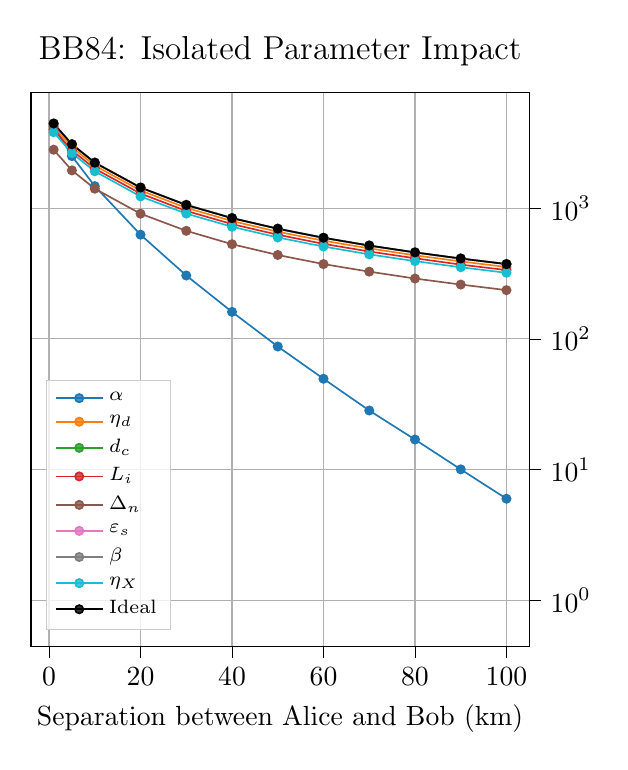
\begin{tikzpicture}

\definecolor{crimson2143940}{RGB}{214,39,40}
\definecolor{darkgray176}{RGB}{176,176,176}
\definecolor{darkorange25512714}{RGB}{255,127,14}
\definecolor{darkturquoise23190207}{RGB}{23,190,207}
\definecolor{forestgreen4416044}{RGB}{44,160,44}
\definecolor{gray127}{RGB}{127,127,127}
\definecolor{lightgray204}{RGB}{204,204,204}
\definecolor{orchid227119194}{RGB}{227,119,194}
\definecolor{sienna1408675}{RGB}{140,86,75}
\definecolor{steelblue31119180}{RGB}{31,119,180}

\begin{axis}[
width=180pt,
height=200pt,
scale only axis,
legend cell align={left},
legend style={
  fill opacity=0.8,
  draw opacity=1,
  text opacity=1,
  at={(0.03,0.03)},
  anchor=south west,
  draw=lightgray204,
  font=\fontsize{7}{9}\selectfont
},
log basis y={10},
tick align=outside,
xtick pos=left,
ytick pos=right,
yticklabel pos=right,
tick label style={font=\fontsize{10}{12}\selectfont},
label style={font=\fontsize{10}{12}\selectfont},
title style={font=\fontsize{12}{14}\selectfont},
title={BB84: Isolated Parameter Impact},
x grid style={darkgray176},
xlabel={Separation between Alice and Bob (km)},
xmajorgrids,
xmin=-3.95, xmax=104.95,
xtick style={color=black},
xtick={-20,0,20,40,60,80,100,120},
xticklabels={
  \(\displaystyle {\ensuremath{-}20}\),
  \(\displaystyle {0}\),
  \(\displaystyle {20}\),
  \(\displaystyle {40}\),
  \(\displaystyle {60}\),
  \(\displaystyle {80}\),
  \(\displaystyle {100}\),
  \(\displaystyle {120}\)
},
y grid style={darkgray176},
ymajorgrids,
ymin=0.443301364171667, ymax=7669.68788693672,
ymode=log,
ytick style={color=black},
ytick={0.01,0.1,1,10,100,1000,10000,100000},
yticklabels={
  \(\displaystyle {10^{-2}}\),
  \(\displaystyle {10^{-1}}\),
  \(\displaystyle {10^{0}}\),
  \(\displaystyle {10^{1}}\),
  \(\displaystyle {10^{2}}\),
  \(\displaystyle {10^{3}}\),
  \(\displaystyle {10^{4}}\),
  \(\displaystyle {10^{5}}\)
}
]
\addplot [semithick, steelblue31119180, mark=*, mark size=1.5, mark options={solid}]
table {%
1 4266.99571014964
5 2511.66927885868
10 1479.33595006783
20 628.504288469735
30 306.042640031697
40 161.141952132203
50 87.5081530118951
60 49.5306050167203
70 28.3176094207888
80 16.9691793887077
90 10.0321492846874
100 5.97592258694378
};
\addlegendentry{$\alpha$}
\addplot [semithick, darkorange25512714, mark=*, mark size=1.5, mark options={solid}]
table {%
1 4230.47200517161
5 2939.92417123343
10 2125.8333981757
20 1370.00124315029
30 1009.29395231607
40 799.966011577559
50 661.604198607232
60 565.424029311353
70 493.732759921548
80 436.628933852052
90 392.426562506118
100 355.366457620532
};
\addlegendentry{$\eta_d$}
\addplot [semithick, forestgreen4416044, mark=*, mark size=1.5, mark options={solid}]
table {%
1 4451.51322372002
5 3092.47851326823
10 2239.93851619128
20 1440.55237144747
30 1064.29139932319
40 842.74254031126
50 697.146533677883
60 593.593781340545
70 519.681419942834
80 460.199011400283
90 412.802896580504
100 374.787620385064
};
\addlegendentry{$d_c$}
\addplot [semithick, crimson2143940, mark=*, mark size=1.5, mark options={solid}]
table {%
1 4017.20522661576
5 2782.09660146099
10 2012.69582353087
20 1297.93781721941
30 955.670950887743
40 757.739673467122
50 627.876945087656
60 534.55718838353
70 467.27912998577
80 414.709678590565
90 370.734382465293
100 336.703536797807
};
\addlegendentry{$L_i$}
\addplot [semithick, sienna1408675, mark=*, mark size=1.5, mark options={solid}]
table {%
1 2811.67818552378
5 1952.85370629832
10 1413.83938950333
20 909.80484214915
30 672.662511706845
40 531.459283646146
50 439.43849736673
60 374.320245173455
70 327.575123074079
80 290.107510917362
90 260.865095741708
100 236.454044222183
};
\addlegendentry{$\Delta_n$}
\addplot [semithick, orchid227119194, mark=*, mark size=1.5, mark options={solid}]
table {%
1 4450.60545165836
5 3094.91065338412
10 2238.08805704181
20 1441.8948878367
30 1064.5067542568
40 842.461624045501
50 697.359896647178
60 595.270172532748
70 517.823636540284
80 459.122599843308
90 413.033623075156
100 374.518229318916
};
\addlegendentry{$\varepsilon_s$}
\addplot [semithick, gray127, mark=*, mark size=1.5, mark options={solid}]
table {%
1 4453.13036284821
5 3088.59282515464
10 2239.92646562033
20 1441.93441800965
30 1061.52191625666
40 842.403339967528
50 698.528562586208
60 595.332283740145
70 518.5245341504
80 459.34137402635
90 412.169642903558
100 375.721438820098
};
\addlegendentry{$\beta$}
\addplot [semithick, darkturquoise23190207, mark=*, mark size=1.5, mark options={solid}]
table {%
1 3827.49930685585
5 2647.94387887145
10 1921.85658308543
20 1233.567010018
30 911.211091740266
40 722.569787109335
50 598.341860802059
60 509.991720190896
70 444.041056180145
80 394.341373539045
90 353.851559719215
100 321.046689111433
};
\addlegendentry{$\eta_X$}
\addplot [semithick, black, mark=*, mark size=1.5, mark options={solid}]
table {%
1 4459.56504885016
5 3095.76002476549
10 2236.80415656955
20 1442.63068926725
30 1060.65402002194
40 841.337125479087
50 698.470185494619
60 595.2023681253
70 518.731111799088
80 460.076861223566
90 412.76957137867
100 374.013990604724
};
\addlegendentry{Ideal}
\end{axis}

\end{tikzpicture}
